
\documentclass[10pt,journal,letterpaper,compsoc]{IEEEtran}

% *** CITATION PACKAGES ***
%
\ifCLASSOPTIONcompsoc
  % IEEE Computer Society needs nocompress option
  % requires cite.sty v4.0 or later (November 2003)
  % \usepackage[nocompress]{cite}
\else
  % normal IEEE
  \usepackage{cite}
\fi
% cite.sty was written by Donald Arseneau
% V1.6 and later of IEEEtran pre-defines the format of the cite.sty package
% \cite{} output to follow that of IEEE. Loading the cite package will
% result in citation numbers being automatically sorted and properly
% "compressed/ranged". e.g., [1], [9], [2], [7], [5], [6] without using
% cite.sty will become [1], [2], [5]--[7], [9] using cite.sty. cite.sty's
% \cite will automatically add leading space, if needed. Use cite.sty's
% noadjust option (cite.sty V3.8 and later) if you want to turn this off.
% cite.sty is already installed on most LaTeX systems. Be sure and use
% version 4.0 (2003-05-27) and later if using hyperref.sty. cite.sty does
% not currently provide for hyperlinked citations.
% The latest version can be obtained at:
% http://www.ctan.org/tex-archive/macros/latex/contrib/cite/
% The documentation is contained in the cite.sty file itself.
%
% Note that some packages require special options to format as the Computer
% Society requires. In particular, Computer Society  papers do not use
% compressed citation ranges as is done in typical IEEE papers
% (e.g., [1]-[4]). Instead, they list every citation separately in order
% (e.g., [1], [2], [3], [4]). To get the latter we need to load the cite
% package with the nocompress option which is supported by cite.sty v4.0
% and later. Note also the use of a CLASSOPTION conditional provided by
% IEEEtran.cls V1.7 and later.





% *** GRAPHICS RELATED PACKAGES ***
%
\ifCLASSINFOpdf
  % \usepackage[pdftex]{graphicx}
  % declare the path(s) where your graphic files are
  % \graphicspath{{../pdf/}{../jpeg/}}
  % and their extensions so you won't have to specify these with
  % every instance of \includegraphics
  % \DeclareGraphicsExtensions{.pdf,.jpeg,.png}
\else
  % or other class option (dvipsone, dvipdf, if not using dvips). graphicx
  % will default to the driver specified in the system graphics.cfg if no
  % driver is specified.
  \usepackage[dvips]{graphicx}
  % declare the path(s) where your graphic files are
  % \graphicspath{{../eps/}}
  % and their extensions so you won't have to specify these with
  % every instance of \includegraphics
  % \DeclareGraphicsExtensions{.eps}
\fi
% graphicx was written by David Carlisle and Sebastian Rahtz. It is
% required if you want graphics, photos, etc. graphicx.sty is already
% installed on most LaTeX systems. The latest version and documentation can
% be obtained at: 
% http://www.ctan.org/tex-archive/macros/latex/required/graphics/
% Another good source of documentation is "Using Imported Graphics in
% LaTeX2e" by Keith Reckdahl which can be found as epslatex.ps or
% epslatex.pdf at: http://www.ctan.org/tex-archive/info/
%
% latex, and pdflatex in dvi mode, support graphics in encapsulated
% postscript (.eps) format. pdflatex in pdf mode supports graphics
% in .pdf, .jpeg, .png and .mps (metapost) formats. Users should ensure
% that all non-photo figures use a vector format (.eps, .pdf, .mps) and
% not a bitmapped formats (.jpeg, .png). IEEE frowns on bitmapped formats
% which can result in "jaggedy"/blurry rendering of lines and letters as
% well as large increases in file sizes.
%
% You can find documentation about the pdfTeX application at:
% http://www.tug.org/applications/pdftex





% *** MATH PACKAGES ***
%
\usepackage[cmex10]{amsmath}
\usepackage{amssymb}
\usepackage{amsfonts}

% A popular package from the American Mathematical Society that provides
% many useful and powerful commands for dealing with mathematics. If using
% it, be sure to load this package with the cmex10 option to ensure that
% only type 1 fonts will utilized at all point sizes. Without this option,
% it is possible that some math symbols, particularly those within
% footnotes, will be rendered in bitmap form which will result in a
% document that can not be IEEE Xplore compliant!
%
% Also, note that the amsmath package sets \interdisplaylinepenalty to 10000
% thus preventing page breaks from occurring within multiline equations. Use:
%\interdisplaylinepenalty=2500
% after loading amsmath to restore such page breaks as IEEEtran.cls normally
% does. amsmath.sty is already installed on most LaTeX systems. The latest
% version and documentation can be obtained at:
% http://www.ctan.org/tex-archive/macros/latex/required/amslatex/math/





% *** SPECIALIZED LIST PACKAGES ***
%
%\usepackage{algorithmic}
% algorithmic.sty was written by Peter Williams and Rogerio Brito.
% This package provides an algorithmic environment fo describing algorithms.
% You can use the algorithmic environment in-text or within a figure
% environment to provide for a floating algorithm. Do NOT use the algorithm
% floating environment provided by algorithm.sty (by the same authors) or
% algorithm2e.sty (by Christophe Fiorio) as IEEE does not use dedicated
% algorithm float types and packages that provide these will not provide
% correct IEEE style captions. The latest version and documentation of
% algorithmic.sty can be obtained at:
% http://www.ctan.org/tex-archive/macros/latex/contrib/algorithms/
% There is also a support site at:
% http://algorithms.berlios.de/index.html
% Also of interest may be the (relatively newer and more customizable)
% algorithmicx.sty package by Szasz Janos:
% http://www.ctan.org/tex-archive/macros/latex/contrib/algorithmicx/




% *** ALIGNMENT PACKAGES ***
%
%\usepackage{array}
% Frank Mittelbach's and David Carlisle's array.sty patches and improves
% the standard LaTeX2e array and tabular environments to provide better
% appearance and additional user controls. As the default LaTeX2e table
% generation code is lacking to the point of almost being broken with
% respect to the quality of the end results, all users are strongly
% advised to use an enhanced (at the very least that provided by array.sty)
% set of table tools. array.sty is already installed on most systems. The
% latest version and documentation can be obtained at:
% http://www.ctan.org/tex-archive/macros/latex/required/tools/


%\usepackage{mdwmath}
%\usepackage{mdwtab}
% Also highly recommended is Mark Wooding's extremely powerful MDW tools,
% especially mdwmath.sty and mdwtab.sty which are used to format equations
% and tables, respectively. The MDWtools set is already installed on most
% LaTeX systems. The lastest version and documentation is available at:
% http://www.ctan.org/tex-archive/macros/latex/contrib/mdwtools/


% IEEEtran contains the IEEEeqnarray family of commands that can be used to
% generate multiline equations as well as matrices, tables, etc., of high
% quality.


%\usepackage{eqparbox}
% Also of notable interest is Scott Pakin's eqparbox package for creating
% (automatically sized) equal width boxes - aka "natural width parboxes".
% Available at:
% http://www.ctan.org/tex-archive/macros/latex/contrib/eqparbox/





% *** SUBFIGURE PACKAGES ***
%\ifCLASSOPTIONcompsoc
%\usepackage[tight,normalsize,sf,SF]{subfigure}
%\else
%\usepackage[tight,footnotesize]{subfigure}
%\fi
% subfigure.sty was written by Steven Douglas Cochran. This package makes it
% easy to put subfigures in your figures. e.g., "Figure 1a and 1b". For IEEE
% work, it is a good idea to load it with the tight package option to reduce
% the amount of white space around the subfigures. Computer Society papers
% use a larger font and \sffamily font for their captions, hence the
% additional options needed under compsoc mode. subfigure.sty is already
% installed on most LaTeX systems. The latest version and documentation can
% be obtained at:
% http://www.ctan.org/tex-archive/obsolete/macros/latex/contrib/subfigure/
% subfigure.sty has been superceeded by subfig.sty.


%\ifCLASSOPTIONcompsoc
%  \usepackage[caption=false]{caption}
%  \usepackage[font=normalsize,labelfont=sf,textfont=sf]{subfig}
%\else
%  \usepackage[caption=false]{caption}
%  \usepackage[font=footnotesize]{subfig}
%\fi
% subfig.sty, also written by Steven Douglas Cochran, is the modern
% replacement for subfigure.sty. However, subfig.sty requires and
% automatically loads Axel Sommerfeldt's caption.sty which will override
% IEEEtran.cls handling of captions and this will result in nonIEEE style
% figure/table captions. To prevent this problem, be sure and preload
% caption.sty with its "caption=false" package option. This is will preserve
% IEEEtran.cls handing of captions. Version 1.3 (2005/06/28) and later 
% (recommended due to many improvements over 1.2) of subfig.sty supports
% the caption=false option directly:
%\ifCLASSOPTIONcompsoc
%  \usepackage[caption=false,font=normalsize,labelfont=sf,textfont=sf]{subfig}
%\else
%  \usepackage[caption=false,font=footnotesize]{subfig}
%\fi
%
% The latest version and documentation can be obtained at:
% http://www.ctan.org/tex-archive/macros/latex/contrib/subfig/
% The latest version and documentation of caption.sty can be obtained at:
% http://www.ctan.org/tex-archive/macros/latex/contrib/caption/




% *** FLOAT PACKAGES ***
%
%\usepackage{fixltx2e}
% fixltx2e, the successor to the earlier fix2col.sty, was written by
% Frank Mittelbach and David Carlisle. This package corrects a few problems
% in the LaTeX2e kernel, the most notable of which is that in current
% LaTeX2e releases, the ordering of single and double column floats is not
% guaranteed to be preserved. Thus, an unpatched LaTeX2e can allow a
% single column figure to be placed prior to an earlier double column
% figure. The latest version and documentation can be found at:
% http://www.ctan.org/tex-archive/macros/latex/base/



%\usepackage{stfloats}
% stfloats.sty was written by Sigitas Tolusis. This package gives LaTeX2e
% the ability to do double column floats at the bottom of the page as well
% as the top. (e.g., "\begin{figure*}[!b]" is not normally possible in
% LaTeX2e). It also provides a command:
%\fnbelowfloat
% to enable the placement of footnotes below bottom floats (the standard
% LaTeX2e kernel puts them above bottom floats). This is an invasive package
% which rewrites many portions of the LaTeX2e float routines. It may not work
% with other packages that modify the LaTeX2e float routines. The latest
% version and documentation can be obtained at:
% http://www.ctan.org/tex-archive/macros/latex/contrib/sttools/
% Documentation is contained in the stfloats.sty comments as well as in the
% presfull.pdf file. Do not use the stfloats baselinefloat ability as IEEE
% does not allow \baselineskip to stretch. Authors submitting work to the
% IEEE should note that IEEE rarely uses double column equations and
% that authors should try to avoid such use. Do not be tempted to use the
% cuted.sty or midfloat.sty packages (also by Sigitas Tolusis) as IEEE does
% not format its papers in such ways.




%\ifCLASSOPTIONcaptionsoff
%  \usepackage[nomarkers]{endfloat}
% \let\MYoriglatexcaption\caption
% \renewcommand{\caption}[2][\relax]{\MYoriglatexcaption[#2]{#2}}
%\fi
% endfloat.sty was written by James Darrell McCauley and Jeff Goldberg.
% This package may be useful when used in conjunction with IEEEtran.cls'
% captionsoff option. Some IEEE journals/societies require that submissions
% have lists of figures/tables at the end of the paper and that
% figures/tables without any captions are placed on a page by themselves at
% the end of the document. If needed, the draftcls IEEEtran class option or
% \CLASSINPUTbaselinestretch interface can be used to increase the line
% spacing as well. Be sure and use the nomarkers option of endfloat to
% prevent endfloat from "marking" where the figures would have been placed
% in the text. The two hack lines of code above are a slight modification of
% that suggested by in the endfloat docs (section 8.3.1) to ensure that
% the full captions always appear in the list of figures/tables - even if
% the user used the short optional argument of \caption[]{}.
% IEEE papers do not typically make use of \caption[]'s optional argument,
% so this should not be an issue. A similar trick can be used to disable
% captions of packages such as subfig.sty that lack options to turn off
% the subcaptions:
% For subfig.sty:
% \let\MYorigsubfloat\subfloat
% \renewcommand{\subfloat}[2][\relax]{\MYorigsubfloat[]{#2}}
% For subfigure.sty:
% \let\MYorigsubfigure\subfigure
% \renewcommand{\subfigure}[2][\relax]{\MYorigsubfigure[]{#2}}
% However, the above trick will not work if both optional arguments of
% the \subfloat/subfig command are used. Furthermore, there needs to be a
% description of each subfigure *somewhere* and endfloat does not add
% subfigure captions to its list of figures. Thus, the best approach is to
% avoid the use of subfigure captions (many IEEE journals avoid them anyway)
% and instead reference/explain all the subfigures within the main caption.
% The latest version of endfloat.sty and its documentation can obtained at:
% http://www.ctan.org/tex-archive/macros/latex/contrib/endfloat/
%
% The IEEEtran \ifCLASSOPTIONcaptionsoff conditional can also be used
% later in the document, say, to conditionally put the References on a 
% page by themselves.




% *** PDF, URL AND HYPERLINK PACKAGES ***
%
\usepackage{url}
% url.sty was written by Donald Arseneau. It provides better support for
% handling and breaking URLs. url.sty is already installed on most LaTeX
% systems. The latest version can be obtained at:
% http://www.ctan.org/tex-archive/macros/latex/contrib/misc/
% Read the url.sty source comments for usage information. Basically,
% \url{my_url_here}.





% correct bad hyphenation here
%\hyphenation{op-tical net-works semi-conduc-tor}


\begin{document}


% can use linebreaks \\ within to get better formatting as desired
\title{Formal Integral Model for\\Creating Virtual Worlds}


% use \thanks{} to gain access to the first footnote area
% a separate \thanks must be used for each paragraph as LaTeX2e's \thanks
% was not built to handle multiple paragraphs
%
%
%\IEEEcompsocitemizethanks is a special \thanks that produces the bulleted
% lists the Computer Society journals use for "first footnote" author
% affiliations. Use \IEEEcompsocthanksitem which works much like \item
% for each affiliation group. When not in compsoc mode,
% \IEEEcompsocitemizethanks becomes like \thanks and
% \IEEEcompsocthanksitem becomes a line break with idention. This
% facilitates dual compilation, although admittedly the differences in the
% desired content of \author between the different types of papers makes a
% one-size-fits-all approach a daunting prospect. For instance, compsoc 
% journal papers have the author affiliations above the "Manuscript
% received ..."  text while in non-compsoc journals this is reversed. Sigh.

\author{Gabriel L\'opez-Garc\'ia,
        Rafael Molina-Carmona, and
        Javier Gallego-S\'anchez% <-this % stops a space
\IEEEcompsocitemizethanks{\IEEEcompsocthanksitem The authors are with the 
Group of Inform\'atica Industrial e Inteligencia Artificial,
Universidad de Alicante, Ap.99, E-03080, Alicante, Spain\protect\\
Tel.: +34 96 590 3400\protect\\
Fax:  +34 96 590 3902\protect\\
E-mail: \{glopez, rmolina, ajgallego\}@dccia.ua.es}}




% The paper headers
\markboth{IEEE TRANSACTIONS ON VISUALIZATION AND COMPUTER GRAPHICS}%
{IEEE TRANSACTIONS ON VISUALIZATION AND COMPUTER GRAPHICS}




% The publisher's ID mark at the bottom of the page is less important with
% Computer Society journal papers as those publications place the marks
% outside of the main text columns and, therefore, unlike regular IEEE
% journals, the available text space is not reduced by their presence.
% If you want to put a publisher's ID mark on the page you can do it like
% this:
%\IEEEpubid{0000--0000/00\$00.00~\copyright~2007 IEEE}
% or like this to get the Computer Society new two part style.
%\IEEEpubid{\makebox[\columnwidth]{\hfill 0000--0000/00/\$00.00~\copyright~2007 IEEE}%
%\hspace{\columnsep}\makebox[\columnwidth]{Published by the IEEE Computer Society\hfill}}
% Remember, if you use this you must call \IEEEpubidadjcol in the second
% column for its text to clear the IEEEpubid mark (Computer Society jorunal
% papers don't need this extra clearance.)



% for Computer Society papers, we must declare the abstract and index terms
% PRIOR to the title within the \IEEEcompsoctitleabstractindextext IEEEtran
% command as these need to go into the title area created by \maketitle.
\IEEEcompsoctitleabstractindextext{%
\begin{abstract}
Virtual Reality (VR) and graphical systems have achieved a wide importance in many fields. The processes of rendering, the physics engines and the artificial intelligence modules have reached a certain maturity. Nevertheless, they are usually defined as separated modules, and there is not a complete model that allows the definition of a whole VR system, including complex interaction.

In this paper, an integrated model to create Virtual Worlds is presented. It integrates the diversity of the VR systems and the main modules: Graphics, Physics and Artificial Intelligence engines. Through the use of a formal grammatical model, a system with the following features is defined: independent from the interaction devices, flexible, complete and reusable. The main elements of the system are primitives, transformations and actors, which use events to communicate.

A case of study is also included: a simulation of fires in forests caused by lightning. This example illustrates the modelling, expansion, and portability of the system, as well as the independence from hardware and the main aspects of graphical representation.
\end{abstract}

% IEEEtran.cls defaults to using nonbold math in the Abstract.
% This preserves the distinction between vectors and scalars. However,
% if the journal you are submitting to favors bold math in the abstract,
% then you can use LaTeX's standard command \boldmath at the very start
% of the abstract to achieve this. Many IEEE journals frown on math
% in the abstract anyway. In particular, the Computer Society does
% not want either math or citations to appear in the abstract.


\begin{IEEEkeywords}
Virtual Reality, Virtual Worlds generation, Formal model, Interaction
\end{IEEEkeywords}}



\maketitle


% To allow for easy dual compilation without having to reenter the
% abstract/keywords data, the \IEEEcompsoctitleabstractindextext text will
% not be used in maketitle, but will appear (i.e., to be "transported")
% here as \IEEEdisplaynotcompsoctitle\documentclass[12pt,journal,compsoc]{IEEEtran}abstractindextext when compsoc mode
% is not selected <OR> if conference mode is selected - because compsoc
% conference papers position the abstract like regular (non-compsoc)
% papers do!
\IEEEdisplaynotcompsoctitleabstractindextext
% \IEEEdisplaynotcompsoctitleabstractindextext has no effect when using
% compsoc under a non-conference mode.


% For peer review papers, you can put extra information on the cover
% page as needed:
% \ifCLASSOPTIONpeerreview
% \begin{center} \bfseries EDICS Category: 3-BBND \end{center}
% \fi
%
% For peerreview papers, this IEEEtran command inserts a page break and
% creates the second title. It will be ignored for other modes.
\IEEEpeerreviewmaketitle



%___________________________________________________________________________
% Computer Society journal papers do something a tad strange with the very first section heading:

\ifCLASSOPTIONcompsoc
  \noindent\raisebox{2\baselineskip}[0pt][0pt]%
  {\parbox{\columnwidth}{\section{Introduction}\label{sec:introduction}%
  \global\everypar=\everypar}}%
  \vspace{-1\baselineskip}\vspace{-\parskip}\par
\else
  \section{Introduction}\label{sec:introduction}\par
\fi
%___________________________________________________________________________


\IEEEPARstart{I}{n} recent years, the development of Virtual Reality (VR) and graphical systems has been amazing.
This progress has contributed to the creation of new ways to analyze and work with information, such
as graphics, animations or simulations. Computer games industry is one of the elements which has
contributed most to the advance of graphical systems and to the emergence of new VR systems.
However, these developments have opened up new challenges.

One of the most important problems is the wide variety of visual devices (monitors, PDAs, cell
phones, VR goggles), each one with different features. For that reason, it is necessary to develop
adaptive systems which generate the images according to the specific characteristics of the device
(resolution, size, ...).

While the processes of visualization and renderization of images have reached a certain maturity in
the past decades, in the field of interaction a similar evolution has not been produced
\cite{Joshua2004,David2005}. Keyboard and mouse still dominate the world of interactive devices.
High degree-of-freedom input devices are complex to manage, and other possibilities of interaction
are only used in research and graphic art \cite{Joshua2004}. However, there has been tentative
progress in recent years. Among them, it can be highlighted the input device of Wii
\cite{wiiNintendo}.

It is necessary to develop a model which unifies the whole range of devices of interaction and
visualization. For example, the action of moving an object in the virtual world, should not be
connected with the push of a specific button on a mouse, a keyboard, or any other device. Instead,
this diversity of events should be unified in one action: ``move the object'', removing this way
all the specific characteristics of the different devices.

In the development of VR systems, there are three major modules which have had an uneven evolution. These are the Graphics, the Physics and the Artificial Intelligence (AI) engines. The first one handles the display of data into visual devices. The second one simulates all the physical processes, providing more coherent actions and visual effects to the virtual world. The last one tries to simulate an intelligent and independent behaviour of the actors in the scene.

There are multiple tools and solutions used to develop these three modules. However, there is not any unified criteria to deal with the different development challenges. There are some common points used to define certain structural designs, but there is no study about the connections between the different modules.

This paper presents a new model which integrates the diversity of the VR systems and the
aforementioned modules (Graphics, Physics and AI engines). The major goal is to
separate the scene definition from the hardware-dependent characteristics of the system devices. It
uses a grammar definition which integrates activities, visualitation and interaction with users.

The following section describes the background of VR systems. Section \ref{sec:objectives} shows
the main objectives to achieve. Section \ref{sec:model} defines the proposed model, and Section
\ref{sec:case_study} presents a case of study. Finally, the conclusions and the lines for future
work are shown.



%___________________________________________________________________________
\section{Background
\label{sec:background}}
%___________________________________________________________________________

A VR system can be considered to be composed of three main modules: render system, physics engine
and AI system. Next, the background of these modules are reviewed briefly.

There are two main libraries which are used to develop components of graphics engines: Direct3D
\cite{DirectX} and OpenGL \cite{OpenGL}. Both libraries are defined as a layer between the
application and the graphics card. Different systems which try to unify these two APIs
(\textit{Aplication Program Interfaces}) into a single interface have appeared. This is the case of
OGRE \cite{OGRE} and VTK \cite{VTK}. There are also libraries which are used to manage the
interactive hardware. Two examples are SDL \cite{SDL} and DirectX \cite{DirectX}. In general, they
have similar features, but SDL is open source and cross-platform.

There are a large variety of tools which implement physics engines, such as Working Model
\cite{WModel} (used mainly in the area of education to perform simulations), Newton Game
Dynamics \cite{NGDynamics}, Physics Abstraction Layer (PAL) \cite{PAL} (it is an open source and cross-platform API for physical simulation), Open Dynamics Engine (ODE) \cite{ODE} (it is an implementation of a part of the PAL specifications), and so on.  There are many other API among the proprietary software, such as PhysX \cite{Physx} (developed by NVidia
and used in the PlayStation 3) and Havok \cite{Havok} (it belongs to the company Havok and it is
implemented for Windows, MacOS, Linux, Xbox 360, Wii, Playstation3 and PlayStation Portable).

The last type are the tools used to develop the AI engine. There are very few libraries which can
be used as a generic solution because they are designed specifically for particular applications.
One of the reasons why the AI systems have been developed more slowly than the rest, may be that
the effort being done to improve the graphical aspects of games is not comparable to the one done
for the improvement of the intelligence of its characters \cite{Laird2001}. Nevertheless, some
types of systems can be found, such as evolutive algorithms or agent-based systems.

There are some tools which facilitate the use of evolutive algorithms, such as EO Evolutionary
Computation Framework \cite{EOECF} (it is implemented in C++ and it has all the necessary to work
with evolutive algorithms), CILib \cite{CILib} (it is a development environment implemented in
Java). There are also a lot of papers about genetic algorithms and about the development of
evolutive algorithms for specific cases \cite{Georgios2004,Chris2007,Robert2005}.

A wide research has been done in the area of agent systems, such as in
\cite{Wooldridge1997,Wood2000}. Currently, these systems are widely used in research for the
development of AI, game characters (called \textit{bots}, especially in first person games), social
simulations and mobile robots \cite{John2007,Kenyon2006}. There are different frameworks which
simplify the task of \textit{bots} development, but they are often oriented to specific games:
QuakeBot for Quake game and FlexBot for Half-Life game \cite{Laird2001,Aaron2002}, for instance.
There are other libraries for the development of generic agents, such as Jade \cite{Jade} (used to
develop multi-agent-based applications).




%___________________________________________________________________________
\section{Objectives
\label{sec:objectives}}
%___________________________________________________________________________

Our objectives are primarly focused on achieving a model which unifies all the modules of a VR
system. This system must be independent of hardware devices, both visual and interaction devices.
It means that one device can be replaced by another one, or even by a simulation, without affecting
the internal mechanisms of the system. To achieve this, the following objectives are proposed:

\begin{enumerate}
    \item Define a graphics engine which eliminates the diversity in visual
devices. That is, only one description is needed to process the scene for any graphical device with
a level of detail according to its features.

    \item Provide flexibility to the graphics system in order to be
able to change the elements of representation. This way, the system can
provide different types of information without the need to modify the scene
description.

    \item Design a graphics system which can be used to extract and use the
elements that are defined in the scene. In addition, it is intended to handle other non-visual
elements like sound.

    \item Define a physics engine which models the whole system activity
and can be adapted to different hardware devices. If there are hardware components which implement
physics algorithms, the system must exploit them, but if not, it should be implemented with
software.

    \item Design a physics engine which can provide the information needed by the graphics system at any time. It is intended to perform functions of simulation and analysis of the elements that compose the scene.

    \item Provide to the physics engine the ability to modify the scene
elements through simulations, but without the need to know the architecture of these elements in
detail.

    \item Unify the AI system with the physics engine. The limitations
imposed by the physics engine must be considered by the AI system.

    \item Make the interaction independent from the hardware. The system has to abstract the origin of the action and process the orders directly from the user. Therefore, the interaction could be handled as an internal process of the system (such as the calculation of collisions).

    \item Design and implementing the elements so that they can be reused. If, for
example, an item is designed for a specific virtual world, it should be able to
be reused in another virtual world or VR application.

    \item Control the activity of the system through events. However, the origin of these events could not be known.

\end{enumerate}


For the fulfillment of these objectives, mathematical models are used to formalize the different
components of the system, abstracting the characteristics of the three major modules of a VR
system.





%___________________________________________________________________________
\section{Model for Virtual Worlds Generation
\label{sec:model}}
%___________________________________________________________________________

A virtual world can be described as an ordered sequence of primitives, transformations and actors.
The concept of primitive is considered as an action executed in a certain
representation system. It is not, for instance, just a primitive to draw a sphere or a cube.
Instead, it could implement any action which could be carried out in a representation device, such
as a sound, for example. Transformations modify the behavior of primitives. Actors are the components which define the activities of the system in the virtual world. They will be displayed through primitives and transformations. To model the different actor's activities, the concept of event is used. Events
are not generated by any certain input device. They are considered as an action that represents the
activation of a certain activity and they can be run by one or more actors.

Each element in the scene is represented by a symbol from the so called ``set of symbols of the
scene''. They are used to build strings to describe scenes. These strings are formed using
a language syntax, which is usually presented as a grammar \cite{Davis1994}. This grammar
(hereafter denoted by $M$) is defined by the tuple $M= \ <\Sigma, N, R, s>$, where $\Sigma$ is a
finite set of terminal symbols used to build strings, $N$ is a finite set of non-terminal symbols
or variables which represents the substrings of this language, $R$ is a finite set of syntactic
rules used to describe how a non-terminal symbol can be defined as a function of terminal and
non-terminal symbols (a syntactic rule is an application $r$: $W^* \rightarrow W^*$, where $W =
\Sigma \cup N$) and $s \in N$ and it is the initial symbol or axiom of the grammar.

Considering the previous definition, $M$ can be defined, in our case, as the following grammar:

\begin{enumerate}
    \item Let $\Sigma = P \cup T \cup O \cup A^D$ be the set of terminal symbols, where:

    \begin{itemize}
        \item $P$ is the set of symbols which defines primitives.

        \item $T$ is the set of symbols which defines transformations.

        \item $O = \{ \cdotp ( ) \}$ is the set of symbols of separation
and operation. () indicates the scope of the previous symbol, and $\cdotp$ the concatenation of
symbols.

        \item $A^D$ is the set of symbols which represents actors. $D$
is the set of all the types of events which are generated by the system. Actors
will carry out activities when they receive one of these events. For example,
the actor $a^d$ will carry out the activity $d$ when it
receives the event $e^d$.
    \end{itemize}



    \item Let $N$ = \{WORLD, OBJECTS, OBJECT, ACTOR, TRANSFORMATION,
FIGURE \} be the set of non-terminal symbols.

    \item Let $s =$ WORLD be the initial symbol of the grammar.

    \item Grammar rules $R$ are defined in Table 1.

\end{enumerate}



\begin{table}[h]
\caption{Grammar rules $R$}
\label{tab:rules}
\begin{center}
\begin{tabular}{|ll|}
    \hline

    Rule 1. & \textbf{WORLD} $\rightarrow$ OBJECTS \\

    Rule 2. & \textbf{OBJECTS} $\rightarrow$ OBJECT $|$ OBJECT · OBJECTS \\

    Rule 3. & \textbf{OBJECT} $\rightarrow$ FIGURE $|$ TRANSFORMATION $|$ \\
            & $|$ ACTOR \\

    Rule 4. & \textbf{ACTOR} $\rightarrow$ $a^d$ (OBJECTS), $a^d \in \textbf{A}^D$ \\

    Rule 5. & \textbf{TRANSFORMATION} $\rightarrow t$ (OBJECTS), $t \in T$ \\

    Rule 6. & \textbf{FIGURE} $\rightarrow$ $p^+$, $p \in P$ \\

    \hline
\end{tabular}
\end{center}
\end{table}



A string $w \in \Sigma^*$ is generated by the grammar $M$ if it can be
obtained starting with the initial symbol WORLD and using the rules of the
grammar. The language generated by the grammar $M$ is the set of all the strings
which can be generated by this method. This language is called $L(M)$ and is
defined as:


\begin{equation}
 L(M) = \lbrace w \in \Sigma^* \ | \ \text{WORLD} \stackrel{*}{\rightarrow} w
\rbrace
\end{equation}


The grammar $M$ is a context-independent grammar (or a type-2 grammar, according to the Chomsky
hierarchy). Therefore, there is a procedure which verifies if a scene is correctly described or, in
other words, if a string belongs to the language $L(M)$ or not. For example, it can be determined
that the string $a_1^d ( p_1 \cdot p_2) \cdot p_3 \cdot t_1 ( p_1 \cdot p_2 ) \in L(M)$ where $p_i
\in P$, $t_i \in T$, $a_i^d \in A^D$, $d \in D$, but, on the contrary, $a_1^d \cdot p_1 \notin
L(M)$.


Apart from the language syntax, it is necessary to define the functionality of the strings, that is,
the semantics of the language. It can be denoted through three methods:
operational, denotational and axiomatic. The first one uses abstract machine language
operations. The second one uses mathematical functions to describe the meaning of the strings. The
third one defines the meaning of the string through mathematical logic terms. In our case, the
denotational method is used.



%___________________________________________________________________________
\subsection{Semantics of the Language $L(M)$
\label{sec:semantic}}

In this section, a mathematical function is assigned to each rule of Table 1.


%___________________________________________________________________________
\subsubsection{Semantic Function for Primitives (Rule 6)
\label{sec:rule6}}

Rule 6 defines the syntax of a figure as a sequence of primitives. Primitive's semantics is defined
as a function $\alpha$. Each symbol in the set $P$ carries out a primitive on a given geometric
system $G$. Therefore, the function $\alpha$ is an application defined as:

\begin{equation}
    \alpha: P \rightarrow G
\end{equation}


So, depending on the definition of the function $\alpha$ and on the geometry of $G$, the result of the
system may be different. $G$ represents the actions which are run on a specific geometric system.

A usual example of geometric system are graphical libraries, such as OpenGL or Direct3D. In this
case, each symbol of $P$ would have associated an action of the render system. For instance, given
the symbol of a sphere ($sphere \in P$), it would implement a function which draws this object in
the corresponding graphics system (Direct3D or OpenGL):

\[ \begin{tabular}{l}
$\alpha_{opengl}(sphere) = glutSolidSphere$ \\
$\alpha_{direc3d}(sphere) = drawSphereDirect3D$
\end{tabular} \]


These functions are examples of visual geometric systems. But this definition can also be extended
to non-visual geometric systems. For example, a non-visual system could be the calculation of the
boundaries of a figure, which could be used to calculate collisions between elements. So, a new
function $\alpha_{bounds}(sphere) = boundSphere$ can be defined for the same alphabet $P$, where
``\textit{boundSphere}'' is a function which calculates the limits of spheres.

Previous examples show that the function $\alpha$ provides the
abstraction needed to homogenize the different implementations of a render
system. Therefore, only a descriptive string is needed to run the same scene on
different graphics systems.

So far, only Euclidean geometric systems have been considered. But, the function $\alpha$ has no
restrictions on the geometric system that can be applied as long as there is a definition for this
primitive. Thus, it could also implement a sound, the movement of a robot, the reflection of a
material and so on. Moreover, the definition of the function $\alpha$ could also describe systems
to write different file formats (VRML, DWG, DXF, XML, etc.), to send strings in a network, etc.




%___________________________________________________________________________
\subsubsection{Semantic Function for Transformations (Rule 5)
\label{sec:rule5}}

Rule 5 defines the syntax for transformations. The scope of a transformation is
limited by the symbols ``()''. Two functions are used to describe the semantics
of a transformation. These functions are:

\begin{equation}
\begin{tabular}{l}
    $\beta: T \rightarrow G$ \\
    $\delta: T \rightarrow G$
\end{tabular}
\end{equation}


$\beta$ represents the beginning of the transformation. It is carried out when the symbol ``('' is
processed and it has to take into account the previous symbol of the set $T$. The function $\delta$
defines the end of the transformation which has previously been activated by the function $\beta$.
It is carried out when the symbol ``)'' is found.

These two functions have the same features that the function $\alpha$, but they
are applied to the set of transformations $T$, using the same geometric system
$G$.

A new function $\varphi$ is defined using the set of primitives $P$, the set
of transformations $T$ and the functions $\alpha$, $\beta$ and $\delta$. Given a
string $w \in L(M)$ and using only symbols of $P$ and $T$, this function
$\varphi$ runs the sequence of primitives and transformations in the geometric
system $G$. It is defined as:

\begin{equation}
    \varphi (w) = \left\{
    \begin{array}{ll}
        \alpha(w) & \mathit{if} \ w \in P  \\

        \beta(t); \varphi(v); \delta(t) & \mathit{if} \ w = t(v) \wedge v \in L(M) \wedge\\
                                        & \wedge \ t \in T \\

        \varphi(s); \varphi(v)  & \mathit{if} \ w = s \cdotp v \wedge s, v \in L(M)
    \end{array}\right\}
\end{equation}


One of the most important features of this system is the independence from a specific graphics
system. The definition of the functions $\alpha$, $\beta$ and $\delta$ provides the differences in
behaviour. These functions encapsulate the implementation details which may differ for different
systems, such as a render system, a geometric calculation system, a command execution system in a
production chain, and so on. Therefore, in the development of strings to define virtual worlds is
not necessary to consider the special features of the geometric system. In addition, these strings
may be used on all the systems which implement these functions.



%___________________________________________________________________________
\subsubsection{Semantic Function for Actors (Rule 4)
\label{sec:rule4}}

Rule 4 of the grammar $M$ refers to actors, which are the dynamic part of the system. The semantics
of the actor is a function which defines its evolution in time. For this reason, the semantic
function is called \textit{evolution function} $\lambda$ and it is defined as:


\begin{equation}
    \lambda: L(M) \times E^D \rightarrow L(M)
\end{equation}

where $E^D$ is the set of events for the device $D$ and the strings $w \in L(M)$ fulfill the
syntactic rule 4. The function $\lambda$ can be interpreted as the evolution of the actor in time.
$\lambda$ has a different expression depending on its evolution over time. However, the
general expression can be defined as:


\begin{equation}
    \lambda (a^{d}(v),e^{f})=
    \left\{
    \begin{array}{ll}
        u \in L(M) & \mathit{if}  \ \ f = d \\
        a^{d}(v)  & \mathit{if}  \ \ f \neq d
    \end{array}\right\}
\end{equation}


It means that an actor $a^{d}(v)$ is transformed into another string $u$ when the actor is prepared
to respond to the event $d$ (that is, $f=d$) and it remains unchanged when it is not
prepared to respond to this event.


The result of the function $\lambda$ may contain or not the own actor, or it can generate other
event for the next stage (or the next frame). So, an actor can become a generator of events. The
new events generated by actors are accumulated to be passed to the next stage of the system
evolution. In this way, a feedback process is generated. Such process is very important for the
physics engine and the AI system.

The function $\lambda$ can define a recursive algorithm which, given a set of
events and a string, describes the evolution of the system at a given point
in time. This function is called \textit{function of the system evolution} and
it is represented by $\eta$. Its definition requires a set of events
$e^i, e^j, e^k, \dots, e^n$, which in short is denoted as $e^v$, where $v
\in D^+$. This algorithm is defined as:


\begin{equation}
    \eta (w, e^v) = \left\{
    \begin{array}{ll}
        w   & \mathit{if}  \ \ w \in P  \\

        t(\eta (v, e^v))    & \mathit{if}  \ \  w = t(v)  \\

        \underset{\forall f \in v}{ \prod }(\lambda (a^d (\eta
            (y, e^v)), e^f))    & \mathit{if}  \ \ w = a^d(y)
\\

        \eta (s, e^v) \cdot \eta (t, e^v)   & \mathit{if}  \
\  w = s \cdot t
    \end{array}\right\}
\end{equation}



The operator $\underset{\forall f \in v}{ \prod }(\lambda (a^d (\eta (y, e^v)), e^f))$ concatenates
the strings generated by the function $\lambda$. It is important to note that the strings which are
only composed of transformations and primitives are not processed. Therefore, these strings are not
part of the system evolution. This fact is important for the system optimization, because the
evolution is carried out only for the strings which contain actors, that is, the dynamic part of
the system.

The functions $\lambda$ can be classified in accordance with the strings which are obtained during
the evolution of the system. One important type of $\lambda$ functions are those which return
strings with only primitives and transformations, because they are essential to define the
visualization of strings. As it was explained before, the functions $\alpha$, $\beta$ and $\delta$ do
not admit strings with actors. Therefore, actors must be first converted into strings made up only
of primitives and transformations. This conversion is carried out by a type of function $\lambda$
called \textit{visualization function}, or function $\theta$, which is defined as:

\begin{equation}
    \theta: L(M) \times E^V \rightarrow L(M')
\end{equation}


where $V \subseteq D$, $E^V$ are events created in the visualization process, and $L(M')$
is the language $L(M)$ without actors. The expression of the visualization function is defined as:


\begin{equation}
    \theta (a^d(v), e^f) =
    \left\{
    \begin{array}{ll}
        w \in L(M') &  \ \ \mathit{if}  \ \ f = d \wedge d \in V \\
        \epsilon  &  \ \ \mathit{if}  \ \ f \neq d
    \end{array}\right\}
\end{equation}



There are small differences between $\lambda$ and $\theta$. The first one is that $\theta$ returns
strings belonging to $L(M')$. The second is that $\theta$ returns an empty string if the event does
not match. So, the actor will not have representation for that event.

The type of event $V$ (visualization event) does not correspond to any specific input device. It is used
to create different views of the system. For example, to design a system which filters
out certain elements in order that they become invisible, it is only necessary to avoid reacting to
those events. Moreover, they can also be used to change the visualization type, depending on the
type of window, or on the output device and its features.

As with the function $\lambda$, an algorithm is defined for $\theta$. It returns a string $z \in
L(M')$, given a string $w \in L(M)$ and a set of events $e^v$, where $v \in V^+$ and $V \subseteq
D$. This function is called \textit{function of system visualization} $\pi$ and it is defined as:


\begin{equation}
   \begin{array}{c}
    \pi: L(M) \times E^V \rightarrow L(M') \\
\\
    \pi (w, e^v) = \left\{
    \begin{array}{ll}
        w   & \mathit{if}  \ \ w \in P^+  \\

        t(\pi (y, e^v))     & \mathit{if}  \ \  w = t(y)  \\

        \underset{\forall f \in v}{ \prod }(\theta (a^v (\pi
            (y, e^v)), e^f))    & \mathit{if}  \ \ w = a^v(y)
\\

        \pi (s, e^v) \cdot \pi (t, e^v)    & \mathit{if}  \
\  w = s \cdot t
    \end{array}\right\} \\
   \end{array}
\end{equation}


This function is the same as the function $\eta$ unless that $\lambda$ is
replaced by $\theta$, and that events can only belong to $V$. If the event does
not belong to $V$, the function $\pi$ returns an empty string.





%___________________________________________________________________________
\subsubsection{Semantic Functions for OBJECT, OBJECTS and WORLD (Rules 1,
2 and 3)
\label{sec:rules123}}

The semantic function of these rules breaks down strings and converts them into substrings. The
functions specified above are carried out depending on whether the symbol is an actor, a
transformation or a primitive. Therefore, the semantic function of WORLD is a recursive function
which breaks down the string of the WORLD and converts it into substrings of OBJECTS. Then, these
substrings are in turn broken down into substrings of OBJECT. And for each substring of OBJECT,
depending on the type of the object, the semantic function of ACTOR, PRIMITIVE or TRANSFORMATION is
run.




%___________________________________________________________________________
\subsection{Activity and Events
\label{sec:activity_events}}

In VR systems some mechanisms must be established to model the activity of the graphics system.
This activity can appear during the action of an actor, between several actors with a certain
relationship (for example, an actor which is composed of other actors -which are their children-
and there is some activity between them), and between input devices and scene's strings. Each type
of activity is different, but they have some features in common, and they are going to be
established.

As it has been said before, actors activity is carried out when a certain type of event is produced
with some specific data. But not all activities are directly run when an event is received. There
are events that only run its activity when certain conditions are satisfied, depending on the
actor state. This condition is not defined at the object that runs the activity, but at the event.
The following event definition is established:
{\itshape $e_c^d$ is defined as an event of type $d \in D$ with data $e$, which is carried out only when the
condition $c$ is fulfilled.
}

For simplicity, when there is not any condition, that is, {\itshape c=TRUE}, the event is
represented by $e^d$.

Let us notice that the origin of events is not identified. In fact, the origin is not
important, but the event type and its data.



%___________________________________________________________________________
\subsection{Input Devices and Event Generators
\label{sec:input_devices}}

It is necessary to establish the independence between the system and the input devices. So, the
events needed to make the system respond to a set of input devices must be defined. It means that
there may be actions on input devices (buttons, mouse wheel, movements and so on) which generate
one or more events, and others which do not generate any. The input devices need not be only
physical devices, they may be software devices which, depending on the system state, may or may not
generate events. For example, a mouse could be used as input device to move the objects in the
scene. However, there has not to be a mouse event associated to the object; instead, there should be
a generic event of movement associated to the object and the mouse has an event generator which
creates events of movement. On the other hand, an example of software device may be an algorithm
for detecting collisions. In this case, an event can be generated when a collision is detected.


A new function called \textit{event generator} is defined as:
{\itshape Let $C^d(t)$ be a function which creates events of type $d$ at the time instant $t$,
where $d \in D$ and $D$ is the set of event types which can be generated by the system.
}


In the previous definition, it should be noticed that events are generated in the time instant $t$.
It is due to synchronization purpose. It is also possible that $C$ does not create any event at a
given moment.

This definition makes the system independent from the input devices. Thus, event generators can be
created for a mouse, a VR glove, a keyboard or any other input device, and all of them can generate
the same type of events. The most interesting fact about the implementation of the event generator
is that the device-dependent code is encapsulated and separated from the rest.

One problem is that different event generators can create the same type of events. So, a priority
order among event generators must be established to avoid ambiguities. Given two generators $C_i$
and $C_j$ which create the same event, if $i < j$, then the events generated by $C_i$ will have a
higher priority. For example, the following priority order could be established among input
devices: $1st$ joystick, $2nd$ mouse and $3rd$ keyboard. This ambiguity is due to the fact that the
system must be implemented for all the possible devices. If there are several devices, only one
prevail. The priority order can be established using different criteria: the level of immersion
into the system, the ease of use and so on.

The process which obtains the events produced by input devices and their associated event
generators is defined as follows:
{\itshape Let $C^*$ be the set of all the event generators which are associated with input
devices.
}


The function $e(z, e^i)$ which concatenates all the events in a list is defined
as:

\begin{equation}
    e(z, e^i) = \left\{
    \begin{array}{ll}
        z \cdot e^i   &   \mathit{if} \ \ e^i \notin z \\
        z    &   \mathit{if} \ \ e^i \in z
    \end{array}
    \right\}
\end{equation}



The function $E(C^*, t)$ collects all the events from all the generators and accumulates them in a
list. If the event $e^i$ already exists, then it is not inserted in the list. This function is
defined as:


\begin{equation}
    E(C^*, t) = \left\{
    \begin{array}{ll}
        e(z, C_i(t))   &  \mathit{if}  \ \ z = E(C^* - C_i, t) \\
        \epsilon   &  \mathit{if} \ \ C^* = \emptyset
    \end{array}
    \right\}
\end{equation}






%___________________________________________________________________________
\subsection{System Algorithm
\label{sec:system_algorithm}}

Once all the elements involved in the model have been defined, the algorithm which carries out the
entire system can be established. It defines the system evolution and its visualization at every
time instant `$t$' or frame. The algorithm of virtual worlds generation is defined as:


\begin{center}
\begin{tabular}{|ll|}
    \hline

    Step 1. & $w = w_o$ \\

    Step 2. & $t = 0$ \\

    Step 3. & $e^* = E(C^*, t)$ \\

    Step 4. & $e^v =$ events of $e^*$ where $v \in V^+$ \\

    Step 5. & $e^u = e^* - e^v$ \\

    Step 6. & $w_{next} = \eta(w, e^u)$ \\

    Step 7. & $v =  \pi(w, e^v)$ \\

    Step 8. & $g = \varphi(v)$ \\

    Step 9. & $w = w_{next}; \ \ t = t + 1$ \\

    Step 10. & If $w = \epsilon$ then go to step 12 \\

    Step 11. & Go to step 3 \\

    Step 12. & End \\

    \hline
\end{tabular}
\end{center}



Where:

\begin{itemize}
    \item $D$ = \{ Set of all the types of possible events in the system \}.

    \item $V$ = \{ Set of all the types of visual events \} where $V \subseteq D$.

    \item $C^*$ = \{ All the event generators which generate events of type $D$ \}.

    \item $g$ is the output device.

    \item $e^*$ are all the events generated by the system.

    \item $e^v$ are all the events from visual devices. These events are
the input of the visual algorithm $\pi$.

    \item $e^u$ are all the events from non-visual devices. These events
are the input of the evolution algorithm $\eta$.

    \item $w_o$ is the intial string of the system.
\end{itemize}




The first two steps initialize the system. The initial state $w_o$ is
introduced to the system and the first frame is set to 0.

Steps 3, 4 and 5 manage the system events. In Step 3, generators are called to insert all the
events in a list $e^*$. In Steps 4 and 5, events are divided into visual events ($e^v$, which are
the input of the visual algorithm $\pi$) and non-visual events ($e^u$, which are the input of the
evolution algorithm $\eta$).

In Step 6, the evolution algorithm $\eta$ is called with the current string $w$ and the non-visual
events ($e^u$). The output is the string for the next frame or instant.

In Steps 7 and 8, the visualization of the system is performed. First, actors are transformed into
primitive and transformations. Next, the visualization algorithm $\pi$ is called with the visual
events ($e^v$). Finally, the function $\varphi$ is called to display the current state of the
system into the render engine $g$.

In Step 9, the next iteration is prepared. $w$ is assigned to $w_{next}$ and the time instant (or
current frame) is increased in 1.

Step 10 checks if the current string satisfies the condition of completion, that is, if the
following string is empty, then the algorithm ends (Step 12). Otherwise, the algorithm goes to Step
3. Therefore, to finish the main algorithm the function $\eta$ must just return an empty string.
This empty string can be generated by a special event which is created when the system must stop.

It must be noticed that Step 6 can be exchanged with Steps 7 and 8, because they do not share any
data. This feature is very important for the parallel implementation of the algorithm.  So, Step 6
and Steps 7 and 8 can be divided into two parallel tasks. This type of optimization has a
significant impact on the final graphics system, which leads to a faster system performance.

The diagram of the virtual world generation algorithm is shown in Figure \ref{fig:diagram}.



\begin{figure}[htb]
    \centering
    \begin{tabular}{cc}
       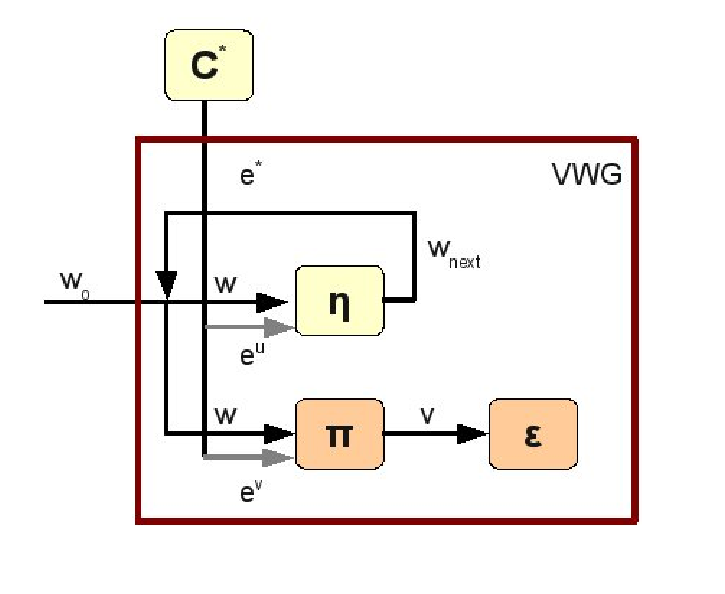
\includegraphics[width=0.8\linewidth]{figure3}
    \end{tabular}
    \caption{\label{fig:diagram} Virtual worlds generation algorithm}
\end{figure}


This formalization of the system has two main consequences. First, the scene definition is
separated from the hardware-dependent characteristics of components. The functions $\alpha$,
$\beta$ and $\delta$ provide the independence from the visualization system, and the event
generators provide the independence from the hardware input devices. Secondly, due to the fact that
there is an specific scheme to define the features of a system, the different system elements can be
reused easily in other areas of application.



%___________________________________________________________________________
\section{Case of Study
\label{sec:case_study}}
%___________________________________________________________________________

This example is an application that simulates fires in forests caused by lightning. It could
be used to analize the best distribution of trees to reduce the number of burnt trees
\cite{John2007}. It is important to notice that we are not actually interested in the problem of fire simulation,
but rather in defining a graphic system using the proposed model and all the concepts presented in
this paper. Therefore, it studies the ease of system modeling, expansion, portability and system
independence from hardware and other aspects of graphical representation.

%___________________________________________________________________________
\subsection{Problem description
\label{sec:description_problem}}
%___________________________________________________________________________

Let $(i, j)$ be the cells of a 2D grid representing a squared world. In each cell, a tree can grow
with a given probability $g$. Bolts of lightning can also fall on a $(i, j)$ position
with a probability $f$. In this case, if there is a tree, it will burn as well as
the trees around it, in a chain reaction. An example can be seen in Figure \ref{fig:ejemplo}.

\begin{figure}[htb]
    \centering
    \begin{tabular}{cc}
        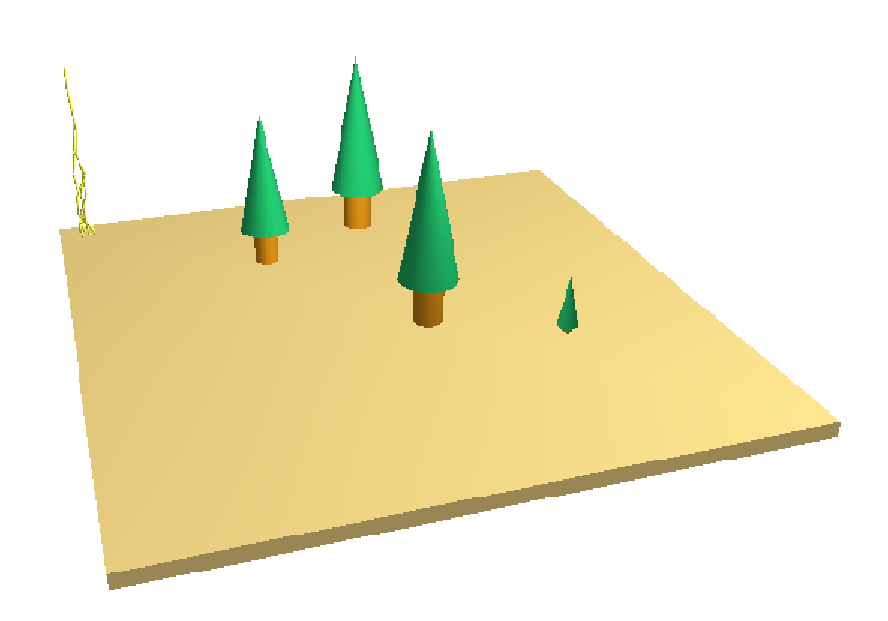
\includegraphics[width=3.5cm]{figure1} &
        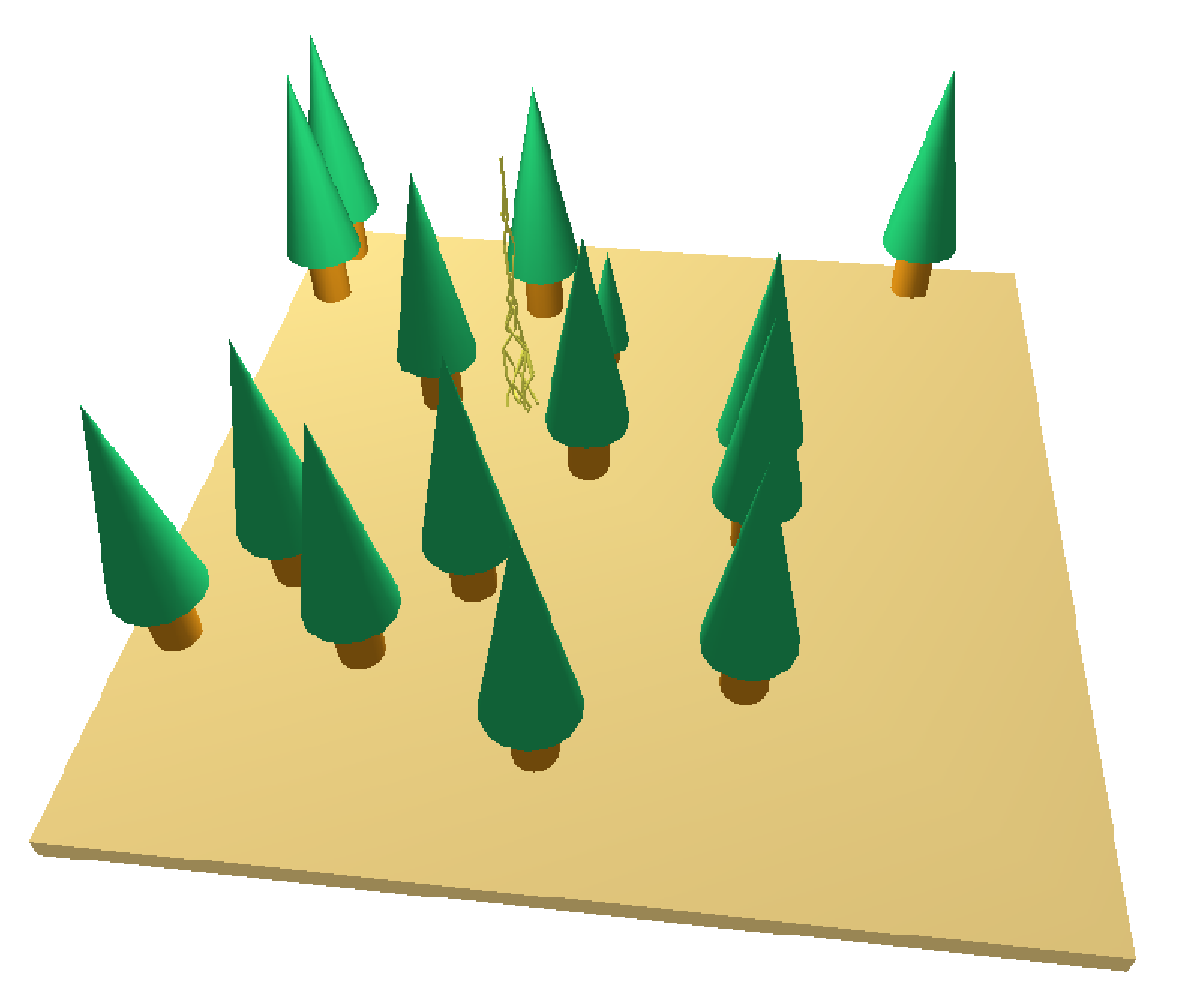
\includegraphics[width=3.5cm]{figure2}
    \end{tabular}
    \caption{\label{fig:ejemplo} Examples of different simulation states}
\end{figure}

To model this example with the Virtual World Generator (VWG), four main elements need to be defined.
First, it is necessary to define events for the system to run actor activities. These events
include the necessary information to develop their activity. Second, it is necessary to design
event generators that separate the interactive system from the origin of the events (mouse, keyboard, and
so on). Third, it is necessary to define the actors included in the scene. These elements are
required for the system to evolve over time. Last, the graphic primitives must be defined to show
the visual elements on the render system.



%___________________________________________________________________________
\subsection{Formalization of the system
\label{sec:formalization_system_model}}
%___________________________________________________________________________

Following the steps described above, the different elements of the system are defined.

%___________________________________________________________________________
\subsubsection{Events
\label{sec:events}}

Events are used to produce the necessary activity of system. They are described by an
identifier and a set of data. Their aim is to produce certain activities of the actors that
compose the scene. The events defined for this example are shown in table \ref{table1}.


\begin{table}[h]
\caption{Events definition}
\label{table1}
\begin{center}
\begin{small}
\begin{tabular}{|p{0.1\linewidth}|p{0.35\linewidth}|p{0.35\linewidth}|}

    \hline
    \itshape Type of event &
    \itshape Meaning &
    \itshape Associated data\\

    \hline
    $t$ &
    Event generated every time instant $t$
    &
    Increasing time since previous event\\

    \hline
    $c$ &
    Create a tree at a given position &
    Position (i,j) where the tree is created \\

    \hline
    $f$ &
    Create a bolt of lightning at a given position &
    Position (i,j) where the bolt of lightning is created\\

    \hline
    $e$ &
    Eliminate the tree at a given position &
    Position (i,j) where the tree is eliminated\\

    \hline
    $b$ &
    Burn the tree at a given position &
    Position (i,j) where the tree to be burned is\\

    \hline
    $v$ &
    Draw using a graphics library (e.g. OpenGL) &
    Void\\

    \hline

\end{tabular}
\end{small}
\end{center}
\end{table}



%___________________________________________________________________________
\subsubsection{Event generators
\label{sec:generators}}

The next step is to define the event generators:

\begin{enumerate}

\item Time event generator:
This generator, named by $C_{time}$, has the responsibility of animating the system. Every time
instant $t$, it generates an event $e^t$ that is usually associated with some type of primitive
transformation to change the appearance of an actor over time.

\item Forest event generator:
This generator produces events to create trees and lightning. Taking into account the
previous specification, trees are created with a probability $g$ and lightning with a probability
$f$. This generator is defined as:

\[C_{forest}=
    \left\{
        \begin{matrix}
            e^{c} & with \ probability \ g \\
            e^{f} & with \ probability \ f
        \end{matrix}\right\}\\ \]

\item Visualization event generator:
This generator is necessary to visualize all the elements in the scene. This means that every
instant time a drawing order is received, the generator captures this order and produces an
event, sending the draw elements of the scene to the graphics system. Its mathematical expression
is given as:

\[C_{visualization} = \{ e^o \ \mathit{each \ drawing \ cycle} \} \]
\end{enumerate}



%___________________________________________________________________________
\subsubsection{Primitives and transformations
\label{sec:primitivesandtransf}}

The primitives and transformations that make up the scene are shown in tables \ref{table2} and
\ref{table3}:

\begin{table}[h]
\caption{Definition of primitives}
\label{table2}
\begin{center}
\begin{small}
\begin{tabular}{|l|l|}

\hline \itshape Primitive & \itshape Description\\
\hline $TR$ & Draw a tree\\
\hline $TR_b$ & Draw a burning tree\\
\hline $FA$ & Draw a bolt of lightning\\
\hline $BO$ & Draw a grid of NxN \\
\hline

\end{tabular}
\end{small}
\end{center}
\end{table}



\begin{table}[h]
\caption{Definition of transformations}
\label{table3}
\begin{center}
\begin{small}
\begin{tabular}{|l|l|}

\hline \itshape Transformations & \itshape Description\\
\hline $D_{i,j}$ & Translate (i,j)\\
\hline $S_{s}$ & Scale (s)\\
\hline

\end{tabular}
\end{small}
\end{center}
\end{table}

The functions ${\alpha}$, ${\beta}$ and ${\delta}$ define these primitives and transformations
and they are implemented with a graphics library (in this case OpenGL). This way, the number of
primitives and transformations can be easily extended just implementing them in the functions
${\alpha}$, ${\beta}$ and ${\delta}$.



%___________________________________________________________________________
\subsubsection{Actors
\label{sec:actors}}

The last step is to specify the actors which compose the dynamic part of the system. As explained in previous sections, an actor is defined by its evolution function $\lambda$. If it has a graphical representation, it also uses the function $\pi$ to generate the primitives and the transformations needed to create that representation. Table \ref{table4} shows the actors defined for this example and their evolution function.


\begin{table}[h]
\caption{Actors defined for this example}
\label{table4}
\begin{small}
\begin{center}
\begin{tabular}{|p{0.18\linewidth}|p{0.7\linewidth}|}

    \hline
    \itshape Actor & \itshape Function ${\lambda}$\\

    \hline 
    \textit{B} \ \ \  \ \ \ \ \ \ \ \ \    Represents the forest &
    $\begin{array}{l}
    \lambda(B^{cfe}, e^{i}) =\\
    \left\{
    \begin{array}{ll}
        TG_c^{t=1} \cdot B^{cfv}       & i = c \\
        F^{t=1}   \cdot B^{cfv}       & i = f \\
        B^{cfe}                        & i = e \\
        B^{cfe}                        & i \neq c,f,e
    \end{array} \right\}
    \end{array}$ \\

    \hline 
	\vspace{-0.1cm}    
    \textit{TG} \ \ \ \ \ \ \ \ \   Represents the growth of a tree &
    $\begin{array}{l}
    \lambda(TG^{t},e^{i}) =\\
    \left\{
    \begin{array}{ll}
        TG^{t+1} & i=t \wedge t+1 \leqslant N_{frames} \\
        T^{b} & i=t \wedge t+1>N_{frames}\\
        TG^{t} & i \neq t
    \end{array}\right\}
    \end{array}$ \\

    \hline \textit{T}  \ \ \  \ \ \  Represents a tree &
    $\begin{array}{l}
    \lambda (T^{b},e^{i}) = \left\{
    \begin{array}{ll}
        TB^{t=1}  & i=b \\
        T^{b} & i\neq b
    \end{array}\right\}
    \end{array}$ \\

    \hline \textit{F} \ \ \  \ \ \  Represents the animation of a bolt of lightning  &
    $\begin{array}{l}
    \lambda (F^{t},e^{i}) =\\
    \left\{
    \begin{array}{ll}
        F^{t+1} & i=t\wedge t+1 \leqslant N \\
        \Delta e^{b}    & i=t\wedge t+1>N_{frames} \\
        F^{t} & i\neq t
    \end{array}\right\}
    \end{array}$ \\

    \hline \textit{TB} \ \ \  Represents a burning tree &
    $\begin{array}{l}
    \lambda(TB^{t},e^{i}) =\\
    \left\{
    \begin{array}{ll}
        TB^{t+1}    & i=t \\
        \Delta e^{e}  & i=t \wedge  t+1>N_{frames} \\
        TB^{t}   & i \neq t
    \end{array}\right\}
    \end{array}$ \\

    \hline

\end{tabular}
\end{center}
\end{small}
\end{table}


Actor $B^{cfe}$ represents the forest. This actor generates a tree or a bolt of lightning if it receives the event $e^{c}$ or the event $e^{f}$ respectively. The event $e^{e}$ only changes the internal state of the actor $B^{cfe}$. It frees its position ($i, j$), so a new tree may grow in the same position.

$TG^{t}$ represents the growth animation of a tree. When the animation ends, that is ($t + 1 > N_{frames}$), the actor $T^{b}$ that represents the new tree is placed in the position ($i, j$). $F^{t}$ is similar to $TG^{t}$, unless it creates a bolt of lightning. When the lightning animation ends, it generates an event $e^{b}$ that burns the tree. This is an example of an actor who becomes an event generator.

$T^{b}$ represents a tree. This actor waits until it receives the event $e^{b}$ and then it turns itself into the actor $TB^{t}$. $TB^{t}$ represents the animation of a burning tree. When the animation ends, that is ($t + 1 > N_{frames}$), it generates an event $e^{e}$ to free the space occupied by the tree.


Table \ref{table5} shows the definition of the drawing function $\pi$. This function is used to obtain the set of primitives and transformations representing the visual aspect of an actor, which is shown on the display.




\begin{table}[h]
\caption{Definition of the drawing function}
\label{table5}
\begin{center}
\begin{small}
\begin{tabular}{|l|l|}

    \hline \itshape Actor & \itshape Function ${\pi}$ \\
    \hline
    $B^{v}$ &
    $\pi (B^{v},e^{i})=\left\{\begin{matrix}\mathit{BO}\hfill\null
        &i=v\hfill\null \\\epsilon \hfill\null &i\neq v\hfill\null
        \end{matrix}\right\}$   \\

    \hline
    $TG^{v}$ &
    $\pi (\mathit{TG}^{v},e^{i})=\left\{\begin{matrix}D_{(i,j)}(S_{s}(\mathit{TR}))\hfill\null
        &i=v\hfill\null \\\epsilon \hfill\null &i\neq v\hfill\null
        \end{matrix}\right\}$   \\

    \hline
    $T^{v}$ &
    $\pi(T^{d},e^{i})=\left\{\begin{matrix}D_{(i,j)}(\mathit{TR})\hfill\null
        &i=v\hfill\null \\\epsilon \hfill\null &i\neq v\hfill\null
        \end{matrix}\right\}$   \\

    \hline
    $F^{v}$ &
    $\pi(F^{d},e^{i})=\left\{\begin{matrix}D_{(i,j)}(\mathit{FA})\hfill\null
        &i=v\hfill\null \\\epsilon \hfill\null &i\neq v\hfill\null
        \end{matrix}\right\}$   \\

    \hline
    $TB^{v}$ &
    $\pi(\mathit{TB}^{v},e^{i})=\left\{\begin{matrix}D_{(i,j)}(S_{s^{-1}}(\mathit{TRB}))\hfill\null
        &i=v\hfill\null \\\epsilon \hfill\null &i\neq v\hfill\null
        \end{matrix}\right\}$   \\

    \hline
\end{tabular}
\end{small}
\end{center}
\end{table}



$S$ represents a growing scale factor which depends on the current state of the actor $TG$. This state is modified by the event $e^{t}$. It causes the effect of tree's growth. The scale value is defined by the expression $s = t / N$, where $N$ is the total number of frames and $t$ is the current instant of time. However, in the case of $TB$ the scale factor is defined as a decreasing scale $s^{-1}$. It causes the effect of a burning tree, which is getting smaller.

The animation of a bolt of lightning is implemented by an algorithm which depends on the instant of time $t$. In general, actors' animations always depend on $t$. It modifies the current state of the actor to change its representation and thus perform the animation.

Finally, the initial string is defined. It is the first string to be processed in the algorithm. From this initial state, the system evolves over time. In this example, it is defined as: $w_{0}=B^{cfe}$





%___________________________________________________________________________
\subsection{View generated by VWG
\label{sec:view_generated}}
%___________________________________________________________________________



This section shows the application implemented for the case of study. Figure \ref{fig:programView}(a) is the initial state of the application, without any frame calculation. However, all the elements (actors, static figures and generators) are ready and with their initial configurations. Figure \ref{fig:programView}(b) shows the animation running. Figures \ref{fig:programView}(c) and \ref{fig:programView}(d) show different system views, they are obtained using the interface's buttons. As can be seen, the application has different menus and action buttons. Theses buttons are used to configurate the visualization view, to manipulate the simulation and to other general options, as for example, close the application.


\begin{figure}[htb]
    \begin{tabular}{cc}
        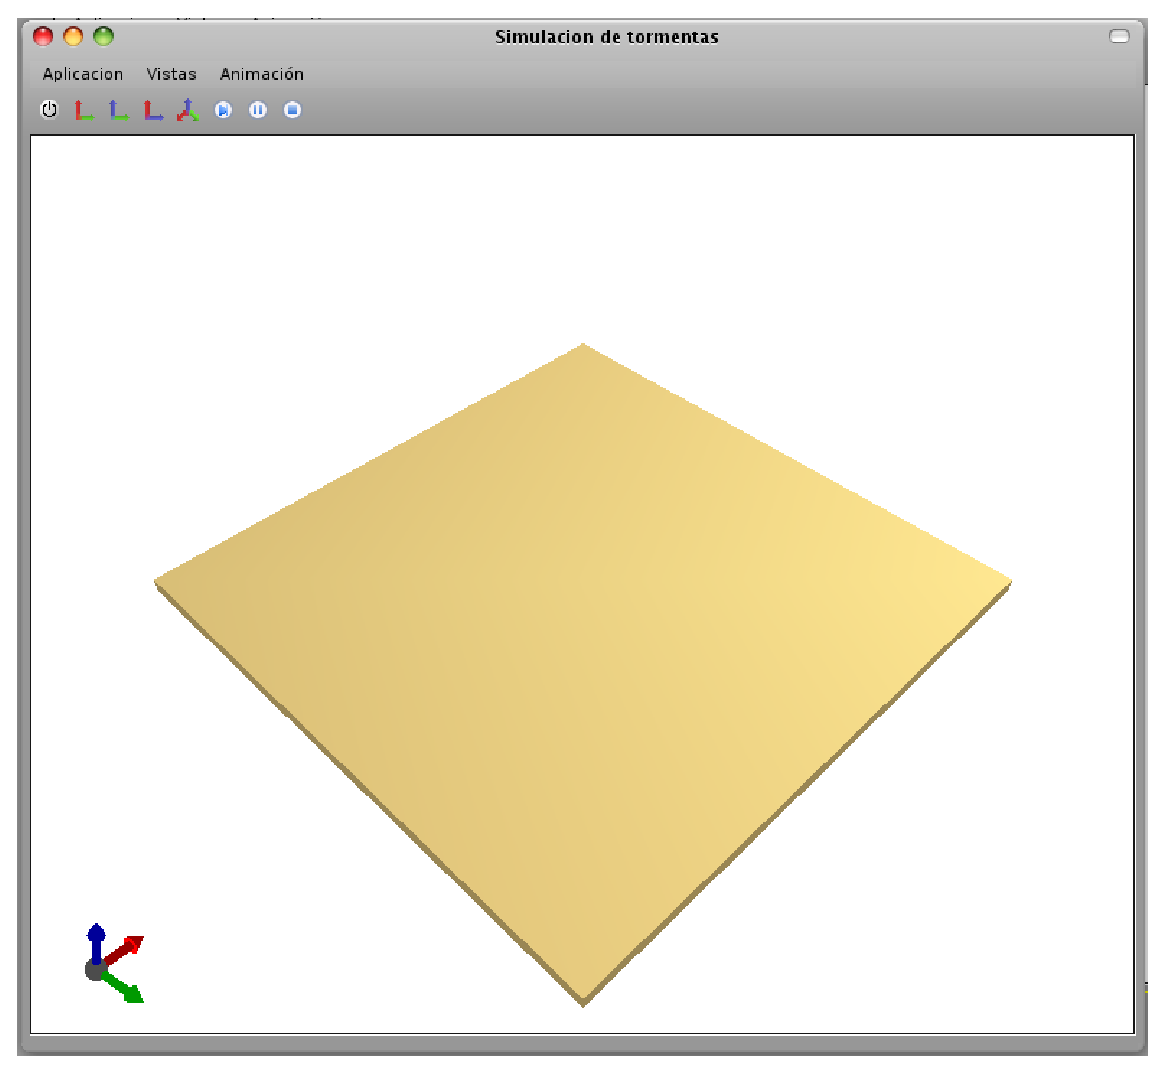
\includegraphics[width=0.45\linewidth]{figure4} &
        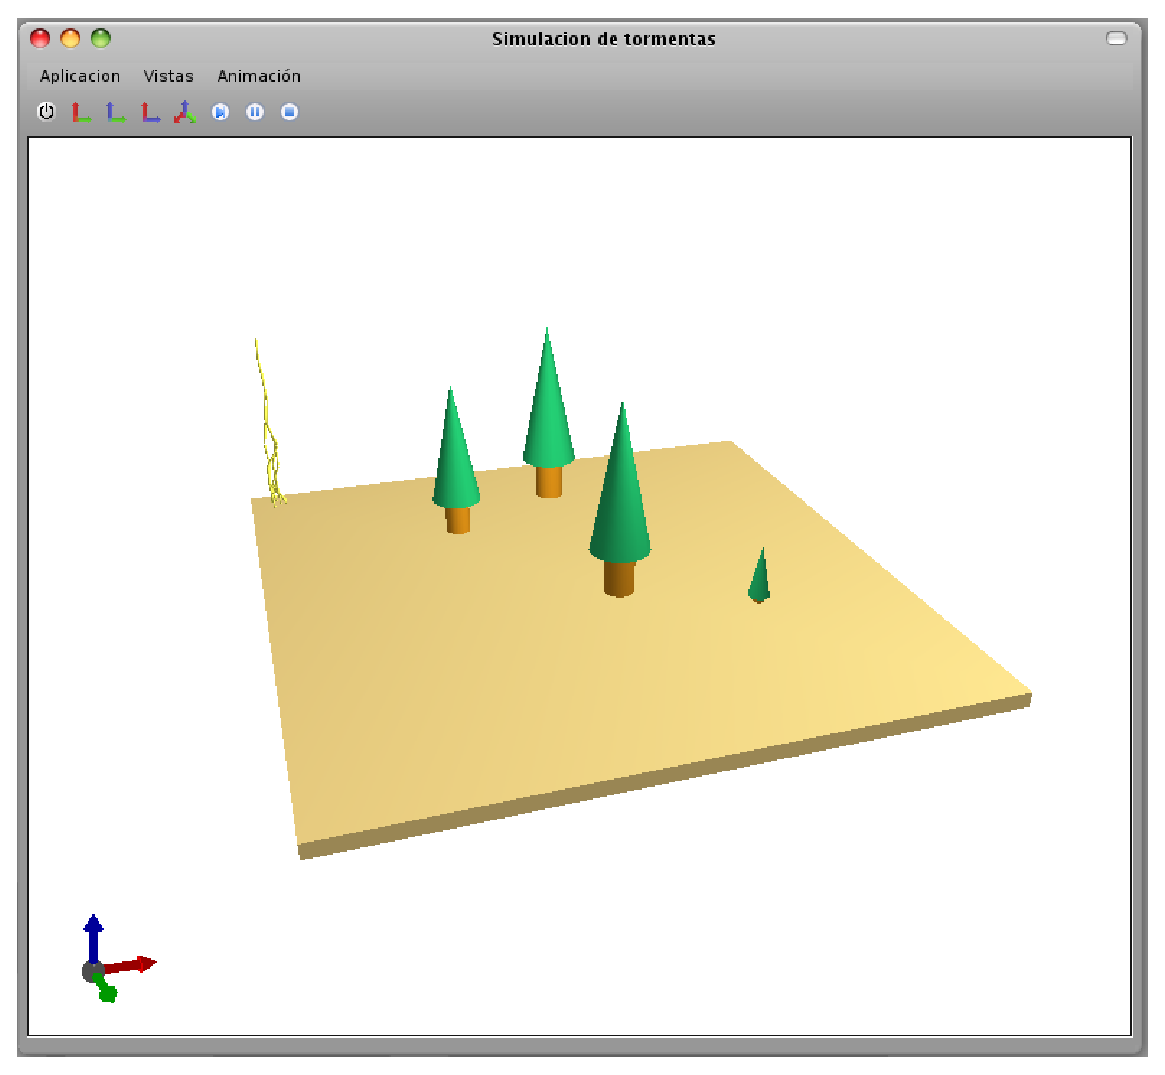
\includegraphics[width=0.45\linewidth]{figure5} \\
        \small{(a)} & \small{(b)} \\
        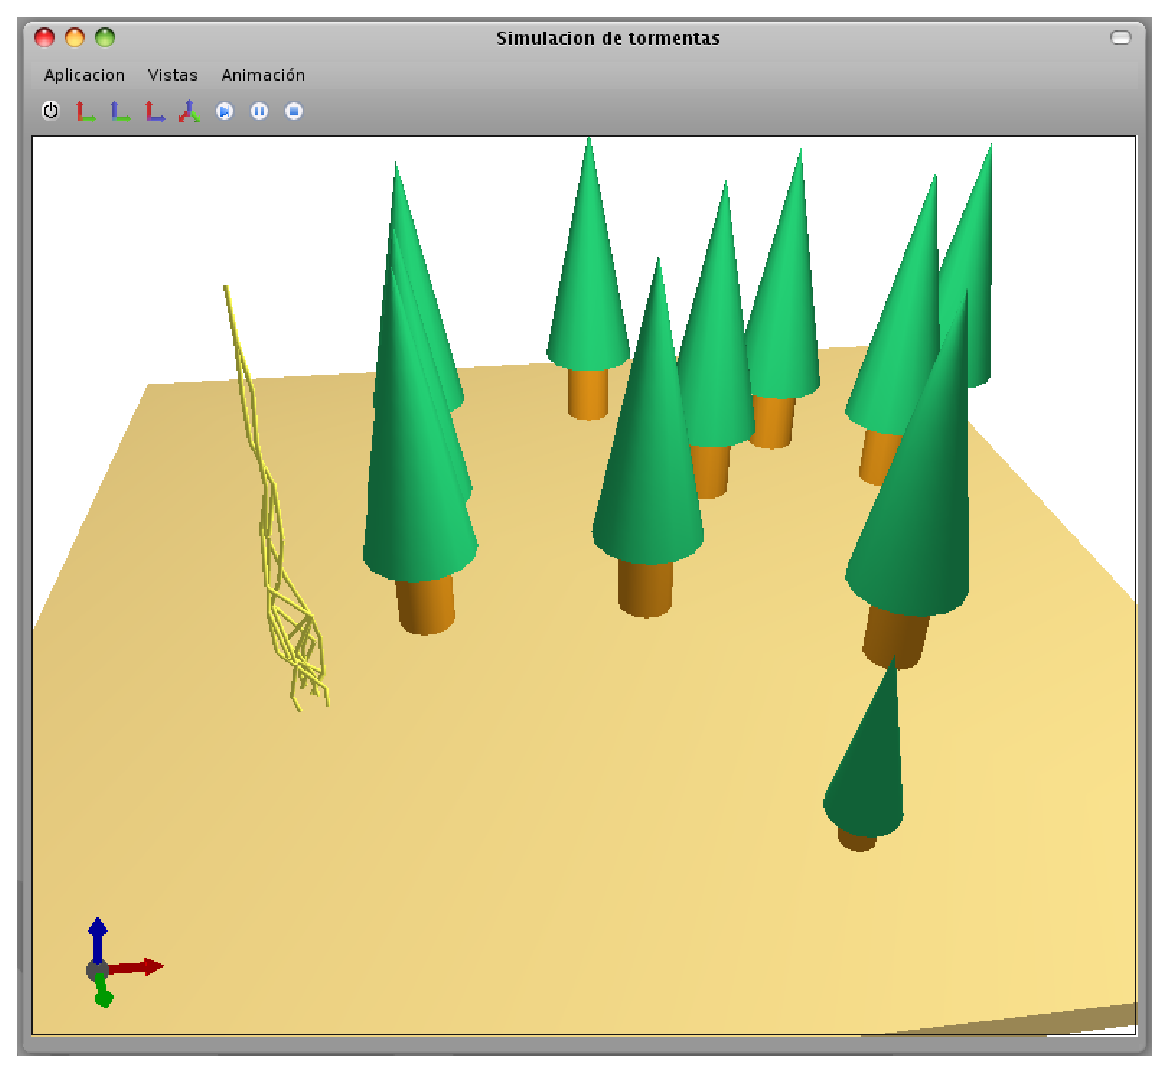
\includegraphics[width=0.45\linewidth]{figure6} &
        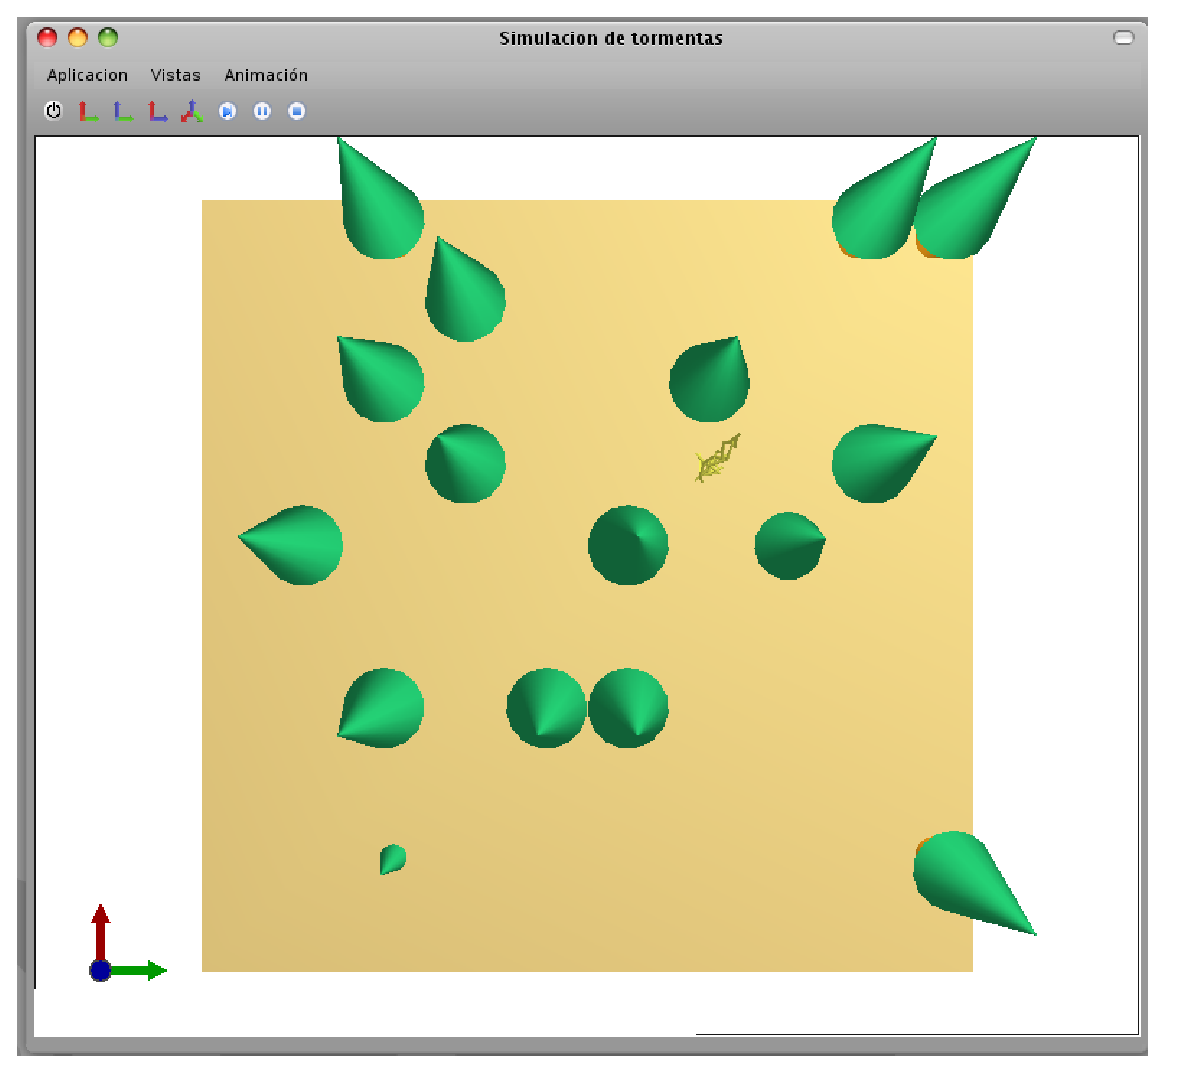
\includegraphics[width=0.45\linewidth]{figure7} \\
        \small{(c)} & \small{(d)} \\
    \end{tabular}
    \caption{\label{fig:programView}
    (a, b) Initial state of the application, (c) Lateral view, (d) XY-view}
\end{figure}




%___________________________________________________________________________
\section{Conclusions and Future Work
\label{sec:conclusions}}
%___________________________________________________________________________

A new model of Virtual Worlds generation has been presented. The major goal of this system is to
separate the scene definition from the hardware-dependent characteristics of the system devices.

First, a language which details the elements of the system using context-free grammars is defined.
Moreover, new functions used to represent the evolution of the elements in time and to extract
their graphic representation are established. This representation is sent to visual devices using
functions which separate the  hardware-dependent implementation of the visual device from the
graphic description of the element. This way, it removes the dependence of the system from the
graphics devices.

The separation of system definition from input devices is made by event generators. These
generators create a layer between the input hardware and the representation of the system. The
actions generated by input devices are linked using the model of events.

In general, the whole model tries to separate the hardware-dependent parts of devices from the
formal definition of a VR system. In order to carry out this separation, different mathematical
models are used to transform device actions, both visual and input devices, into more general
actions. The system must be able to identify these general actions regardless of the origin of the
action. It is achieved using abstraction.

This model has several advantages: firstly, input devices can be replaced by other devices or even
software-simulated devices. Secondly, the different elements of the system can be easily reused.
Thirdly, the representation of the elements can be visual or non-visual, or even it may be
different depending on the display device or the user needs. Thus, if a device has specific
characteristics, the representation can always be adapted to the device. Finally, actors can
interact between them by sending events to each other.

Using the proposed system, new physics engines which use the elements of the scene can be easily
designed. It is achieved by setting up different types of event generators. Depending on the
physical features of the device, it activates the activity of the actor needed to react to that
physical process. For example, if an actor has to react to collisions, the event generator of this
type calculates the collisions between elements by extracting the scene geometry from the graphics
engine (it uses the implementation of the functions $\alpha$, $\beta$ and $\delta$ to calculate the
bounding box of the elements). Then, it generates the events needed to react to such collisions.
This event generator could be implemented with hardware if the system allows it.

The AI engine can be implemented in the evolution function of the actors. Actors use these
functions to make decisions according to their current status. Moreover, events carry out
activities which change the status and the behaviour of actors. As actors can generate events,
it is possible to implement the feedback processes used in AI. The integration between the physics
engine and the AI engine is guaranteed because both engines are connected by events.

The model presented in this work is currently under development. It is pretended to continue
developing several issues. One point to investigate - which is also introduced in this article - is
the optimization of the algorithm and its parallelization. The definition of the system through
strings facilitates the possibility of parallel algorithms. From another point of view, strings
represent the states of the system and its evolution. This evolution may change through mutations,
so different evolutive solutions may be conceived to design new systems. We also consider the
possibility of a new type of events which are activated with a certain probability. For example, if
an actor is defined as $r^{ab}$ and it receives the event $e^a$, then the function associated with
this event will be carried out only with a certain probability.

In conclusion, the main aim has been to design a reusable and generic system, which can be easily
increased, adapted, and improved. It is also important that the core of the system (the evolution
in time) is independent of its representation and the elements which it interacts with.





% use section* for acknowledgement
%--------------------------------------------------------
%\ifCLASSOPTIONcompsoc
  % The Computer Society usually uses the plural form
%  \section*{Acknowledgments}
%\else
  % regular IEEE prefers the singular form
%  \section*{Acknowledgment}
%\fi

%The authors would like to thank...


% Can use something like this to put references on a page
% by themselves when using endfloat and the captionsoff option.
%\ifCLASSOPTIONcaptionsoff
%  \newpage
%\fi



% trigger a \newpage just before the given reference
% number - used to balance the columns on the last page
% adjust value as needed - may need to be readjusted if
% the document is modified later
%\IEEEtriggeratref{8}
% The "triggered" command can be changed if desired:
%\IEEEtriggercmd{\enlargethispage{-5in}}

% references section

% can use a bibliography generated by BibTeX as a .bbl file
% BibTeX documentation can be easily obtained at:
% http://www.ctan.org/tex-archive/biblio/bibtex/contrib/doc/
% The IEEEtran BibTeX style support page is at:
% http://www.michaelshell.org/tex/ieeetran/bibtex/
%\bibliographystyle{IEEEtran}
% argument is your BibTeX string definitions and bibliography database(s)
%\bibliography{IEEEabrv,../bib/paper}
%
% <OR> manually copy in the resultant .bbl file
% set second argument of \begin to the number of references
% (used to reserve space for the reference number labels box)
\begin{thebibliography}{28}

\bibitem{Physx}
\emph{PhysX by AGEIA},
http://physx.ageia.com

\bibitem{David2005}
David J.~Kasik, William~Buxton, D.~R.~Ferguson,
\emph{Ten cad challenges},
IEEE Computer Graphics and Applications 25 (2005), 81--90

\bibitem{WModel}
\emph{Working Model: Simulaci\'on de Sistemas},
http://www.design-simulation.com

\bibitem{Davis1994}
Davis Martin D., ~Sigal R., Weyuker E.~J.:
\emph{Computability, Complexity, and Languages, Fundamentals of Theoretical Computer Science}, 2nd~ed.
San Diego: Elsevier Science, 1994

\bibitem{NGDynamics}
\emph{Newton Game Dynamics},
http://www.newtondynamics.com

\bibitem{ODE}
\emph{Open Dynamics Engine},
http://www.ode.org

\bibitem{Wikipedia2007}
Wikipedia - Physics engine:\\
http://en.wikipedia.org/wiki/physics\_engine

\bibitem{Havok}
Havok:
http://www.havok.com

\bibitem{John2007}
John H.~Miller S. E.~P.:
Complex Adaptative Systems.
Princeton University Press, 2007

\bibitem{Joshua2004}
Joshua~Strickon J. A.~P.:
Emerging technologies.
Siggraph (2004)

\bibitem{PAL}
PAL: Physics Abstraction Layer:
http://www.adrianboeing.com/pal/

\bibitem{DirectX}
Página oficial de DirectX:\\
http://www.microsoft.com/windows/directx/default.mspx

\bibitem{OpenGL}
Página oficial de OpenGL:
http://www.opengl.org/

\bibitem{SDL}
Simple DirectMedia Layer (SDL):
http://www.libsdl.org

\bibitem{OGRE}
OGRE 3D: Open source graphics engine:
http://www.ogre3d.org

\bibitem{VTK}
The Visualization ToolKit (VTK):
http://public.kitware.com/vtk

\bibitem{EOECF}
EO Evolutionary Computation Framework:
http://eodev.sourceforge.net

\bibitem{CILib}
CILib (Computational Intelligence Library):
http://cilib.sourceforge.net

\bibitem{wiiNintendo}
Wii-Nintendo:
http://www.nintendo.es

\bibitem{Jade}
Jade - Java Agent DEvelopment Framework:
http://jade.tilab.com

\bibitem{Laird2001}
Laird J.~E.:
Using a computer game to develop advanced ai.
Computer 34 (7) (2001), 70--75

\bibitem{Georgios2004}
Georgios N.~Yannakakis John~Levine J.~H.:
An evolutionary approach for interactive computer games.
In Proceedings of the Congress on Evolutionary Computation (2004), 986--993.

\bibitem{Chris2007}
Chris~Miles Juan~Quiroz R. L. S. J.~L.:
Co-evolving influence map tree based strategy game players.
IEEE Symposium on Computational Intelligence and Games (2007), 88--95

\bibitem{Robert2005}
Robert G.~Reynolds Ziad~Kobti T. A. K. L. Y. L.~Y.:
Unraveling ancient mysteries: Reimagining the past using evolutionary
  computation in a complex gaming environment.
IEEE transactions on evolutionary computation 9 (2005), 707--720

\bibitem{Wooldridge1997}
Wooldridge M.:
Agent-based software engineering.
IEEE Proceedings Software Engineering 144 (1997), 26--37.

\bibitem{Wood2000}
Wood M.~F., DeLoach S.:
An overview of the multiagent systems engineering methodology.
AOSE (2000), 207--222

\bibitem{Kenyon2006}
Kenyon S.~H.:
Behavioral software agents for real-time games.
IEEE Potentials 25 (2006), 19--25

\bibitem{Aaron2002}
Aaron~Khoo R.~Z.:
Applying inexpensive ai techniques to computer games.
IEEE Intelligent Systems 17(4) (2002), 48--53

\end{thebibliography}



%__________________________________________________________________
%__________________________________________________________________
% biography section
% 
% If you have an EPS/PDF photo (graphicx package needed) extra braces are
% needed around the contents of the optional argument to biography to prevent
% the LaTeX parser from getting confused when it sees the complicated
% \includegraphics command within an optional argument. (You could create
% your own custom macro containing the \includegraphics command to make things
% simpler here.)
%\begin{biography}[{\includegraphics[width=1in,height=1.25in,clip,keepaspectratio]{mshell}}]{Michael Shell}
% or if you just want to reserve a space for a photo:

%\begin{IEEEbiography}{Michael Shell}
%Biography text here.
%\end{IEEEbiography}

% if you will not have a photo at all:
\begin{IEEEbiographynophoto}{Gabriel López-García}
received the B.S. degree in Computer Science from University of Valencia, Spain, in 1990. After that, he received the M.S. degree in Computer Science Engineering from the University of Alicante, Spain, in 2005. He is a PhD student in the Department of Computer Science and Artificial Intelligence in the same university. He has worked as software engineer since 1990 in a CAD-CAE software company. His research interests are in computer graphics and AI Systems, particularly in visualization, virtual reality, interactive system, Multi-Agent system and social behaviour.
\end{IEEEbiographynophoto}

% insert where needed to balance the two columns on the last page with
% biographies
%\newpage

\begin{IEEEbiographynophoto}{Rafael Molina-Carmona}
is a professor in the Department of Computer Science and Artificial Intelligence in the University of Alicante, Spain, which he joined in 1995. He received a B.S. \& M.S. degree in Computer Science from the Polythecnical University of Valencia, Spain, in 1994, and the PhD from the University of Alicante in 2002. His research interests are in computer graphics, computer aided design and manufacturing, artificial vision, 3D reconstruction and virtual reality.
\end{IEEEbiographynophoto}


\begin{IEEEbiographynophoto}{Javier Gallego-Sánchez}
received the B.S. \& M.S. degree in Computer Science Engineering from the University of Alicante, Spain, in 2004. He is a PhD student in the Department of Computer Science and Artificial Intelligence in the same university. His research interest is in computer graphics, particularly in artificial vision, visualization, 3D reconstruction and virtual reality.
\end{IEEEbiographynophoto}


% You can push biographies down or up by placing
% a \vfill before or after them. The appropriate
% use of \vfill depends on what kind of text is
% on the last page and whether or not the columns
% are being equalized.

%\vfill

% Can be used to pull up biographies so that the bottom of the last one
% is flush with the other column.
%\enlargethispage{-5in}



% that's all folks
\end{document}


